\documentclass[12pt]{article}
\usepackage{geometry}
\usepackage{setspace}
\usepackage{graphicx}
\usepackage{booktabs}
\usepackage{float}
\usepackage[hidelinks]{hyperref}
\usepackage{amsmath}
\usepackage{amssymb}
\usepackage[utf8]{inputenc}
\usepackage{listings}
\usepackage{xcolor}
\usepackage{array}
\usepackage{multirow}
\usepackage[numbers,sort&compress]{natbib}
\geometry{margin=1in}
\setstretch{1.15}

\lstset{
	language=Python,
	basicstyle=\ttfamily\scriptsize,
	backgroundcolor=\color{gray!10},
	frame=single,
	breaklines=true,
	breakatwhitespace=false,
	postbreak=\mbox{\textcolor{red}{$\hookrightarrow$}\space},
	columns=flexible,
	keepspaces=true,
	numbers=left,
	numberstyle=\tiny\color{gray},
	numbersep=5pt,
	showstringspaces=false,
	tabsize=4,
	captionpos=b,
	keywordstyle=\color{blue!70},
	stringstyle=\color{red!60},
	commentstyle=\color{green!50!black}
}

\title{\textbf{EE627 Final Project\\ Stacked Ensemble Music Recommender}}
\author{\textbf{Jude Eschete}\\[0.5em]
	\normalfont\normalsize Source code, all submission CSVs, and run logs:\\
	\normalfont\normalsize \url{https://github.com/JEschete/EE627}}
\date{\today}

\begin{document}

	\maketitle

	\newpage
	%======================================================================
	\section*{Executive Summary}
	%======================================================================

	The final project's stacked ensemble~\citep{wolpert1992stacking} reached a Kaggle public score of $\mathbf{0.922}$, an improvement of $+0.011$ over the midterm production submission ($0.911$) and $+0.008$ over the strongest individual base model from Homework~9 ($0.914$). The final submission is a logistic-regression meta-learner trained on the $6{,}000$ \texttt{test2\_new.txt} labels, fed by twenty-three feature columns drawn from every prior assignment in the semester: Project~1's evidence/genre heuristics, Homeworks~3--7's tuned linear baselines, Homework~8's PySpark MF, Homework~9's seven PySpark classifiers, the midterm's BPR neural ranker, and one new orthogonal base model (item-item collaborative filtering) added in this final.

	Five iterations of the meta-learner were built and submitted. The most important finding is empirical: between v1 and v3 the Kaggle score moved $0.918 \rightarrow 0.919 \rightarrow 0.919$ despite three rounds of meta-learner refinements (regularization tuning, calibration, NDCG@3 cross-validation). The plateau was broken in v4 by adding an item-item collaborative filtering signal that operates on the raw rating-co-occurrence matrix instead of on the same 32-feature representation every other model used. v4 jumped to $0.922$. v5 confirmed v4 by tying it with a tuned multi-variant iicf stack, which validates that the item-item CF signal was the binding constraint, not meta-learner sophistication.

	\newpage
	%======================================================================
	\section{Process and Techniques}\label{sec:process}
	%======================================================================

	\paragraph{Hardware note.} The pipeline runs on a single workstation; CUDA is used opportunistically. Production runs were timed on an NVIDIA RTX~5080 (16~GB, CUDA~12.x), with the GPU accelerating only two stages: the rank-$64$ matrix-factorization training (HW7-style SGD, $\sim\!20\,\text{s}$ on the 5080) and the BPR neural ranker training ($\sim\!90\,\text{s}$). Both modules check \texttt{torch.cuda.is\_available()} at startup and fall back to CPU automatically; the rest of the stack (PySpark ALS, the HW9 classifiers, item-item CF, and every meta-learner) is CPU-only by design. The total wall time for a full end-to-end run with all caches present is under one minute on CPU and under four minutes including GPU training from scratch. Anyone re-running this code on a smaller card or no GPU at all will see longer MF/BPR training times but will reach the same Kaggle score; all randomness is seeded.

	\subsection{Course Techniques Applied}

	The final's pipeline reuses every recommender technique introduced in the semester:

	\begin{itemize}
		\item \textbf{Hand-tuned heuristic scoring (Project~1, midterm v2).} A linear combination of album rating, artist rating, and genre-mean rating served as the production submission for the midterm at Kaggle $0.871$. Used in the final both as a continuous feature (\texttt{v2\_score}, \texttt{v2\_rank}) and as the foundation for the v5 confidence-gated hybrid.
		\item \textbf{Matrix factorization (HW7, HW8).} Stochastic-gradient MF with rank $k=64$ trained on GPU. The user/item embeddings feed a dot-product feature into the BPR neural ranker. The cached factor matrices are reused in every final-project run.
		\item \textbf{PySpark ALS (HW8 / lecture demos).} ALS at rank~20 with default regularization, scoring every $(uid, tid)$ pair against the trained user/item factors. The PySpark Spark-session configuration with \texttt{-Xss32m} thread stacks (carried over from HW8 to handle Windows JVM serialization) is reused verbatim.
		\item \textbf{PySpark.ML supervised classifiers (HW9).} Logistic regression, decision tree, random forest, gradient-boosted tree, and an extra-trees variant were trained on the $6{,}000$ \texttt{test2\_new.txt} labels in HW9. The seven probability columns plus the five hand-built blends from HW9 are the strongest individual signals available---the \texttt{hw9\_consensus} feature receives the largest positive weight in every meta-learner version.
		\item \textbf{Confidence-gated hybrids (midterm).} The midterm's $v5\!+\!v2$ gap-thresholded hybrid sweep (gap $0$ through gap $20$) was kept as eleven binary submission columns, then collapsed into the \texttt{v5b\_hybrid\_consensus} family feature in v2$+$.
		\item \textbf{BPR neural ranker (midterm).} The Bayesian Personalized Ranking loss with thirty-two hand-engineered features per candidate, trained on PyTorch with the GPU. Reused as a continuous feature \texttt{v5\_score} (and its per-user normalized variant \texttt{v5\_rank}).
	\end{itemize}

	The class also introduced \emph{ensemble blending} in Week~12 as the final lecture preview:
	\[
	  \hat{y}_{\text{blend}} = \sum_{k=1}^{K} w_k\, \hat{y}^{(k)},
	\]
	where each $\hat{y}^{(k)}$ is a prior Kaggle submission and $w_k$ are weights that minimize prediction error. The final's meta-learner is exactly this construction, with three additions (Section~\ref{sec:beyondclass}): L2-regularized LR-learned weights, fitted on a held-out labeled set rather than Kaggle, with probability calibration on non-binary inputs.

	\newpage
	\subsection{Past-Submission Ensembling: The Foundation}

	The professor's advice in Week~12 was to \emph{keep every Kaggle submission, regardless of how low the score is}---each one becomes a diversified vote in the eventual ensemble. The final implements this directly. The folder \texttt{past\_predictions/} contains $39$ historical submission CSVs, named with their Kaggle scores so the meta-learner can sort them by quality. Table~\ref{tab:past-prov} maps each submission family to the assignment that produced it.

	\begin{table}[H]
		\centering
		\footnotesize
		\caption{Provenance of the $39$ past-submission columns. Each row's CSVs are loaded as binary $0/1$ feature columns into the meta-learner; v2$+$ collapses families into ``consensus'' rate features.}\label{tab:past-prov}
		\renewcommand{\arraystretch}{1.2}
		\begin{tabular}{@{}l p{0.55\textwidth} p{0.30\textwidth}@{}}
			\toprule
			Source & Submissions kept & Rolled into family \\
			\midrule
			Project~1 & \texttt{p1\_evidence}, \texttt{p1\_weightedavg}, \texttt{p1\_maxgenre} & \texttt{p1\_consensus} \\
			HW3--HW7  & \texttt{v3\_additive}, \texttt{v3\_confidence}, \texttt{v3\_genre\_both}, \texttt{v3\_interact}, \texttt{v3\_tuned}, \texttt{v4\_ridge} & \texttt{v3\_consensus} \\
			HW8       & \texttt{hw8\_hybrid}, \texttt{hw8\_hybrid\_gated}, \texttt{hw8\_pyspark\_mf} & \texttt{hw8\_consensus} \\
			HW9       & 5 hw9 binary blends ($0.913$--$0.914$) plus 7 raw probability columns & \texttt{hw9\_consensus}; HW9 isotonic columns \\
			Midterm   & 11 \texttt{v5b\_hybrid\_gap*}, 8 \texttt{v6\_hybrid\_gap*}, \texttt{v5b\_nn\_0878} & \texttt{v5b\_hybrid\_consensus}, \texttt{v6\_hybrid\_consensus} \\
			\bottomrule
		\end{tabular}
	\end{table}

	The $39$ submissions span four model families (heuristic, MF, neural, gradient-boosted-trees) and six logical generations of code. They are exactly what the Week~12 lecture meant by ``many diverse submissions raise the ceiling.'' The $0.011$ Kaggle improvement from midterm ($0.911$) to final ($0.922$) is mostly attributable to this archive: the meta-learner's largest weight in every version is \texttt{hw9\_consensus} (weights $+2.31, +2.33, +2.30$ in v2/v4/v5 respectively), which is the average of the five $0.913\!-\!0.914$ HW9 blend submissions.

	\newpage
	\subsection{Beyond the Class}\label{sec:beyondclass}

	Four techniques used in the final were not introduced in lectures: LightGBM LambdaRank~\citep{burges2010lambdamart,ke2017lightgbm}, isotonic regression calibration~\citep{zadrozny2002calibration,niculescu2005calibration}, item-item collaborative filtering with cosine similarity~\citep{sarwar2001itemitem,linden2003amazon}, and NDCG@K with grouped cross-validation~\citep{jarvelin2002ndcg}. Of those, only item-item CF moved the Kaggle score; the other three contributed within fold-noise. The role each technique played in the iteration history is detailed in Section~\ref{sec:iterations}; full bibliographic entries appear in the References section.

	\newpage
	%======================================================================
	\section{Starting Point: The HW9 Score and Why It Was the Floor}\label{sec:hw9floor}
	%======================================================================

	HW9's strongest individual classifier (Random Forest with $200$ trees, depth $10$, sqrt feature subset) reached a Kaggle public score of $0.914$, tied with an RF variant trained without the v2 feature and with a rank-averaged blend of four tree models. The HW9 report identified the cause of the plateau: three different tree-family submissions all scored $0.914$ but disagreed on only $2.25\%$ of rows. They were sampling slightly different points on the same Pareto frontier rather than capturing different signals.

	The HW9 report concluded:

	\begin{quote}
		\emph{``Tree ensembles plateau without a different model family. Three tree-based submissions all scored $0.914$ and disagreed on only $2.25\%$ of rows---adding a fourth tree variant won't help. The final's stacked meta-learner therefore consumes nine signal sources spanning four model families.''}
	\end{quote}

	The final picks up exactly there. The HW9 plateau ($0.914$) is the floor the v1 stacker had to clear. The midterm production submission ($0.911$, the v5$+$v2 confidence-gated hybrid at gap $10$) is the second floor.

	\subsection{v1: First Crack at the Plateau}

	The v1 stacker concatenated every available signal into a single $49$-column feature matrix and fit \texttt{sklearn.linear\_model.LogisticRegressionCV} on the $6{,}000$ \texttt{test2\_new.txt} labels with random $5$-fold cross-validation:

	\begin{itemize}
		\item v5 BPR neural-net continuous score
		\item v2 heuristic score
		\item ALS rank-20 score
		\item 7 HW9 probability columns (lr, dt, rf, gbt, gbt\_cv, rf\_no\_v2, extra)
		\item 39 historical Kaggle submissions as binary $0/1$ columns
	\end{itemize}

	The trained meta-learner reported a 5-fold cross-validated AUC of $\mathbf{0.9860}$, applied the learned weights to all $120{,}000$ test rows, picked top-3 candidates per user, and submitted. \textbf{Kaggle score: $\mathbf{0.918}$, an improvement of $+0.004$ over the best HW9 base model and $+0.007$ over the midterm production.}

	\subsection{Why v1 Cracked the HW9 Floor}

	The HW9 plateau was caused by a single model family (trees) running out of room. v1 broke that by giving the meta-learner access to:

	\begin{itemize}
		\item The HW9 trees themselves (as both binary blends and raw probabilities).
		\item A different model family the trees did not have---the BPR neural ranker (val AUC $0.7424$ on its own group-of-six validation, but Kaggle $0.878$ standalone).
		\item Two heuristic baselines (v2, v3) that tree models had effectively absorbed but that retained complementary error structure when combined linearly.
		\item Eleven midterm hybrid submissions whose binary outputs encode the v5$+$v2 confidence gate at different thresholds.
	\end{itemize}

	{\sloppy The meta-learner's top weights in v1 were \texttt{hw9\_blend\_rank} ($+0.91$), \texttt{hw9\_rf\_no\_v2} ($+0.87$), \texttt{hw9\_rf} ($+0.77$), \texttt{v5b\_nn\_0878} ($+0.67$), \texttt{v2\_score} ($+0.47$), and \texttt{v5\_score} ($+0.45$). The $+0.004$ improvement over the best individual HW9 model is the value of having the BPR neural ranker, the v2/v5 raw scores, and the eleven midterm hybrids voting alongside the trees.\par}

	The early-warning flag in v1 was the gap between the cross-validated AUC ($0.9860$) and the Kaggle score ($0.918$). That $0.07$ gap is much larger than blend stackers usually see. v2 fixed it.

	\newpage
	%======================================================================
	\section{Iteration History}\label{sec:iterations}
	%======================================================================

	Five iterations of the stacker were built. Each version's design choices were driven by inspecting the previous version's weight table, cross-validation behavior, and Kaggle score. Table~\ref{tab:iterations} summarizes them.

	\begin{table}[H]
		\centering
		\small
		\caption{Stacker versions, feature counts, the dominant change at each step, and the resulting Kaggle public score. The CV column reports honest GroupKFold-by-user $5$-fold mean; v1 was random fold and is shown for comparison.}\label{tab:iterations}
		\begin{tabular}{@{}cc p{0.45\textwidth} cc@{}}
			\toprule
			Version & \# feats & Dominant change & CV AUC & Kaggle \\
			\midrule
			v1 & 49 & all-in LR over $39$ binary subs $+$ raw scores & $0.9860^*$ & $0.918$ \\
			v2 & 21 & per-user ranks; family consensus; GroupKFold & $0.9859$ & $0.919$ \\
			v3 & 23 & $+$ LightGBM, isotonic calibration, NDCG@3 & $0.9858$ & $0.919$ \\
			v4 & 23 & $+$ item-item CF (replaces LightGBM) & $\mathbf{0.9873}$ & $\mathbf{0.922}$ \\
			v5 & 25 & 3 tuned iicf variants; ALS dropped & $0.9879$ & $0.922$ \\
			\bottomrule
		\end{tabular}\\
		\smallskip
		{\footnotesize $^*$random $5$-fold; not directly comparable to the GroupKFold rows.}
	\end{table}

	\subsection{v2 --- Honest CV, Per-User Ranks, Family Consensus}

	The v2 changes were diagnostic, not architectural. Four targeted fixes:

	\begin{enumerate}
		\item \textbf{Per-user rank features added.} For each user's six candidates, the highest-scoring tid is mapped to $1.0$ and the lowest to $0.0$. The \texttt{v5\_rank} and \texttt{v2\_rank} columns let the meta-learner see within-user ordering directly. Kaggle scores top-3-of-6, so this is the metric the model should be tuning toward.
		\item \textbf{Family consensus collapse.} The $39$ past submissions cluster into six logical families (\texttt{v5b\_hybrid\_*}, \texttt{v6\_hybrid\_*}, \texttt{hw9\_*}, \texttt{v3\_*}, \texttt{p1\_*}, \texttt{hw8\_*}) whose members agree on $\sim\!95\%$ of rows. Replacing $39$ binary columns with $6$ ``consensus rate'' features (fraction of family voting~$1$) plus $2$ ungrouped one-offs (\texttt{v4\_ridge\_0852}, \texttt{p1\_maxgenre\_0834}) reduces the matrix to $21$ columns.
		\item \textbf{GroupKFold-by-user 5-fold CV.} The v1 CV was random and leaked: each user's six rows were appearing in both train and validation folds, letting the LR memorize per-user patterns. \texttt{sklearn.model\_selection.GroupKFold} fixed this. The honest CV AUC came in at $0.9859$ vs.\ v1's $0.9860$---the leak was tiny in magnitude but the bias direction matters for ablation comparisons.
		\item \textbf{Non-negative least-squares sanity baseline.} A second meta-learner using SciPy's \texttt{nnls} solver on the $16$ core features. NNLS forces all weights $\geq 0$, killing the sign-flip artifacts the v1 LR had used to cancel correlated past submissions.
	\end{enumerate}

	\paragraph{Result.} Kaggle $0.919$ for the LR meta-learner, $0.916$ for the NNLS sanity baseline. NNLS underperforming the LR by only $0.003$ Kaggle points indicates that the LR's negative weights were doing genuine bias-correction across collinear features, not noise-fitting. The v2 weight table is dominated by \texttt{hw9\_consensus} ($+2.31$), \texttt{v2\_score} ($+0.60$), \texttt{v5b\_nn\_0878} ($+0.57$), and \texttt{v5\_score} ($+0.40$). No more $\pm 0.5$ sign-flip noise.

	\paragraph{Lesson.} A $+0.001$ Kaggle lift from four meta-learner-side fixes is small but real. By the end of v2 it was clear we were close to the meta-learner ceiling and that further gains would require a base-model change.

	\newpage
	\subsection{v3 --- LightGBM LambdaRank, Isotonic Calibration, NDCG@3 Tuning}

	v3 introduced three external methods and ablated each so the contribution could be isolated. Ablation submissions were generated for each method individually plus the combined ``ALL'' variant.

	\begin{enumerate}
		\item \textbf{LightGBM LambdaRank}~\citep{burges2010lambdamart,ke2017lightgbm}. Trained on the same $32$ hand-engineered features the BPR neural net uses, with the natural per-user group-of-$6$ structure. Relevance grades $[5,4,3,2,1,0]$ assigned by within-group rating rank. Hypothesis: a tree-based ranker would learn ranking patterns the neural net missed.
		\item \textbf{Isotonic regression calibration}~\citep{zadrozny2002calibration,niculescu2005calibration}. Cross-fitted (5-fold GroupKFold) isotonic calibrators on the v5 BPR continuous score and each of the seven HW9 probability columns. The calibrators re-map raw model outputs onto a common probability scale before stacking.
		\item \textbf{NDCG@3 grouped CV}~\citep{jarvelin2002ndcg}. Replace the LR's AUC-based regularization tuning with NDCG@3 evaluated under GroupKFold-by-user. NDCG@3 is the closest analog of the Kaggle scoring rule (top-3-of-6 within user).
	\end{enumerate}

	\paragraph{Result.} All five v3 ablation variants scored Kaggle $0.919$. The honest CV AUC barely moved (v2 $0.9859$ to v3-ALL $0.9858$). The most informative observation is what the LightGBM ranker did during training:

	\begin{quote}
		\emph{Training LightGBM LambdaRank ($705{,}270$ groups $\times$ 6) ...}\\
		\emph{Early stopping, best iteration is: $[1]$ val's ndcg@3: $0.775247$}\\
		\emph{Saved LightGBM ranker -> lgbm\_lambdarank.txt}
	\end{quote}

	The model early-stopped after a single boosting round. The $32$ hand-engineered features are saturated by the BPR neural network's val AUC of $0.7424$; a tree model trained on the same features cannot extract additional information. The combined feature \texttt{lgbm\_rank\_score} received an essentially-zero weight in the v3 meta-learner.

	Method B (isotonic calibration) moved CV AUC by $+0.0002$. Method C (NDCG@3 tuning) selected a different best-$C$ ($1.0$ instead of $0.1$), but the change in Kaggle was zero. Methods B and C together are clean engineering improvements that did not move the Kaggle score.

	\paragraph{Lesson.} A new model on existing features cannot add information; only a new model on \emph{new features} can. This is the textbook ensemble-diversity result~\citep{caruana2004ensemble} demonstrated empirically. Three rounds of meta-learner refinement (v1$\rightarrow$v2$\rightarrow$v3) produced $+0.001$ total Kaggle lift, which was the meta-learner ceiling for this base-model set.

	\newpage
	\subsection{v4 --- The Item-Item CF Breakthrough}

	v4 added one new base model: item-item collaborative filtering with cosine similarity over the raw rating-co-occurrence matrix~\citep{sarwar2001itemitem,linden2003amazon}. For each test pair $(uid, tid)$, the score is computed as

	\[
		\text{iicf}(uid, tid) = \sum_{j \in \text{Top-30}(uid)} \cos(tid, j) \cdot r_{uid, j},
	\]

	where $\cos(tid, j)$ is the cosine similarity between items $tid$ and $j$ over their co-raters (with a minimum overlap of $5$ shared raters required), and $r_{uid, j}$ is the user's rating on history item $j$. The similarity is computed sparsely from an inverted index built once at startup.

	The crucial design choice is what the iicf signal is built from. Every other base model in the stack uses either pre-aggregated per-pair statistics (album rating, artist rating, genre means, popularity) or learned MF embeddings (the $64$-dim user/item factors from HW7). The item-item CF score uses neither---it is a pure neighborhood method on the raw $295{,}799$-item co-rating graph. This is the ``different feature space'' v3 had been missing.

	\paragraph{Result.} Kaggle $\mathbf{0.922}$, plateau broken. The iicf-only sanity submission (top-3-of-6 per user using only the iicf score) scored Kaggle $0.781$, which is much weaker than the v5 hybrid baseline ($0.911$) but is a healthy standalone score for a pure neighborhood method with no parameter learning.

	The v4 weight table tells the story directly:

	\begin{table}[H]
		\centering
		\caption{Top-10 standardized LR weights in the v4 meta-learner. \texttt{iicf\_rank} ranks $3$rd despite being a brand-new base model.}\label{tab:v4-weights}
		\begin{tabular}{lr}
			\toprule
			Feature & Weight \\
			\midrule
			\texttt{hw9\_consensus}        & $+2.3293$ \\
			\texttt{v2\_score}             & $+0.5805$ \\
			\texttt{iicf\_rank}            & $+0.4740$ \\
			\texttt{v5b\_nn\_0878}         & $+0.4655$ \\
			\texttt{iicf\_score}           & $+0.3240$ \\
			\texttt{dt\_iso}               & $-0.3140$ \\
			\texttt{v5b\_hybrid\_consensus}& $+0.2329$ \\
			\texttt{v6\_hybrid\_consensus} & $+0.2133$ \\
			\texttt{gbt\_iso}              & $+0.2124$ \\
			\texttt{v5\_iso}               & $+0.2123$ \\
			\bottomrule
		\end{tabular}
	\end{table}

	The meta-learner gives iicf $0.80$ of total weight ($0.474 + 0.324$), more than any new method since v2. CV AUC moved $+0.0015$ ($0.9858 \rightarrow 0.9873$), and the Kaggle score moved $+0.003$. CV-to-Kaggle correlation finally held: a $\sim\!2\times$ amplification factor that is normal for a real signal. The flat NDCG@3 was a mild red herring---iicf was reordering boundary candidates near the top-3 cut without changing the very top, an effect AUC catches but NDCG@3 does not.

	\paragraph{The ALS rank=80 sub-experiment.} v4 also bumped PySpark ALS from rank $20$ to rank $80$. The rationale was that rank $20$ scored only $0.621$ standalone in HW8 and received only a $+0.04$ weight in v1; perhaps a higher-rank ALS could be a useful second matrix-factorization signal. The meta-learner disagreed: in v4 \texttt{als\_score} received weight $-0.151$ and \texttt{als\_rank} received $-0.117$. Higher rank made ALS more confident on rows where it was wrong, and the LR was forced to subtract it. v5 reverted this by dropping ALS entirely.

	\paragraph{Lesson.} The single largest single-step gain in the project ($+0.003$) came from a method that operates on a fundamentally different representation of the data. Three rounds of meta-learner sophistication (v2/v3) gave $+0.001$ combined; one round of base-model diversification gave $+0.003$.

	\newpage
	\subsection{v5 --- Tuning the iicf Variants and Dropping ALS}

	v5 used the v4 result as a directional signal and made two follow-up changes:

	\begin{enumerate}
		\item \textbf{Three iicf variants instead of one.} The v4 iicf used $\text{topk}=30$ history items per user and a minimum co-rater requirement of $\text{min\_co}=5$. v5 also computed \texttt{iicf\_b} ($\text{topk}=50, \text{min\_co}=3$, looser similarity threshold) and \texttt{iicf\_c} ($\text{topk}=20, \text{min\_co}=10$, stricter threshold). Each variant contributed a rank and a score column; the meta-learner picked the best mix.
		\item \textbf{ALS dropped entirely.} The negative weights in v4 confirmed ALS was actively hurting the stack. Removing the two ALS columns reduced the feature count from $25$ to $23$ in the variant-controlled sense (or to $25$ from $23$ after adding two new iicf variants).
	\end{enumerate}

	\paragraph{Result.} Kaggle $0.922$, identical to v4. CV AUC inched up to $0.9879$ from v4's $0.9873$; CV NDCG@3 inched down to $0.9632$ from $0.9635$. Both moves are within fold standard deviation, but the ranking is consistent: v5 marginally better on continuous discrimination (AUC), v4 marginally better on within-user top-3 sharpness (NDCG@3).

	The v5 weight table reveals what the variant tuning actually surfaced:

	\begin{table}[H]
		\centering
		\caption{v5 LR weights for the three iicf variants. The looser-threshold variant (\texttt{iicf\_b}) is the dominant signal; the stricter variant (\texttt{iicf\_c}) is actively subtracted as noise.}\label{tab:v5-iicf}
		\begin{tabular}{lcc}
			\toprule
			Variant & rank weight & score weight \\
			\midrule
			\texttt{iicf\_a} (k$=30$, m$=5$, original v4) & $+0.0977$ & $+0.1412$ \\
			\texttt{iicf\_b} (k$=50$, m$=3$, looser)      & $\mathbf{+0.8192}$ & $+0.2395$ \\
			\texttt{iicf\_c} (k$=20$, m$=10$, stricter)   & $-0.3593$ & $-0.1106$ \\
			\bottomrule
		\end{tabular}
	\end{table}

	\texttt{iicf\_b}'s combined weight ($+1.06$) is larger than the entire iicf signal in v4 ($+0.80$). The strict-threshold variant \texttt{iicf\_c} is uninformative noise that the LR had to cancel with negative weights---repeating the same pattern as ALS in v4.

	\paragraph{Lesson.} Tuning the iicf hyperparameters surfaced a real preference (looser similarity thresholds work better on this dataset) without translating into a Kaggle improvement. The plateau at $0.922$ is therefore the genuine ceiling for the current base-model set, not a tuning artifact. v4 and v5 are equivalent submissions; either can serve as the final.

	\newpage
	%======================================================================
	\section{Lessons Learned}\label{sec:lessons}
	%======================================================================

	\subsection{Stacking works best with diverse signals, not more signals}

	v2 reduced the feature count from $49$ to $21$ by collapsing near-duplicate past submissions into family-consensus features---and the Kaggle score went up. The $28$ features that were removed were collinear duplicates the LR had to spend regularization capacity canceling out. More columns is not better when most columns are near-duplicates. The same reasoning explains why \texttt{iicf\_c} hurt v5: it added a column whose error pattern was correlated with \texttt{iicf\_b}, forcing the LR into another sign-flip cancellation.

	\subsection{Honest grouped cross-validation is non-negotiable}

	Random-fold CV on $6{,}000$ rows reported AUC $0.9860$. GroupKFold-by-user on the same data reported $0.9859$. The numerical gap was small, but the bias direction matters: random folds put each user's $6$ rows in both train and validation, allowing per-user pattern memorization. Without GroupKFold, every ablation in v3 onward would have been compared against an inflated baseline. Trusting a leaked CV is the same as not having a CV.

	\subsection{CV-to-Kaggle amplification is roughly $2\times$ for real signals}

	The most useful diagnostic in the project: when v3 added LightGBM, CV AUC moved by $-0.0001$ and Kaggle moved by $0.000$. When v4 added iicf, CV AUC moved by $+0.0015$ and Kaggle moved by $+0.003$. Across all four iterations a real CV AUC change tended to translate to roughly twice the Kaggle change. CV lifts smaller than the fold standard deviation ($\sim\!0.003$) are unlikely to move Kaggle in the third decimal.

	\subsection{Add base models on new features, not new algorithms on old features}

	The cleanest empirical result of the project: LightGBM LambdaRank in v3 was a ``new base model'' on paper, but it trained on the same $32$ features the BPR neural net had already saturated. It early-stopped at iteration~$1$ with NDCG@3 $0.775$ and contributed nothing to the meta-learner. Item-item CF in v4 was also a ``new base model,'' but it operated on the raw $295{,}799$-item co-rating graph---a fundamentally different representation. It produced the project's largest single-step Kaggle gain ($+0.003$).

	\begin{table}[H]
		\centering
		\small
		\caption{The clearest single comparison in the project: same idea (``add a new base model''), opposite outcomes.}\label{tab:lgbm-vs-iicf}
		\begin{tabular}{@{}l p{0.30\textwidth} p{0.40\textwidth}@{}}
			\toprule
			Method & Trained on & Kaggle effect \\
			\midrule
			LightGBM (v3) & Same 32 features as BPR-NN & $0.000$ (saturated, early-stopped at iter 1) \\
			Item-item CF (v4) & Raw 295K-item co-rating matrix & $+0.003$ (broke 3-version plateau) \\
			\bottomrule
		\end{tabular}
	\end{table}

	\subsection{A base model's standalone Kaggle score does not predict its stacking contribution}

	ALS at rank $20$ scored Kaggle $0.621$ standalone---one of the worst submissions in the archive. When promoted to rank $80$ for v4 the standalone behavior improved, but the meta-learner gave both ALS columns negative weights ($-0.151$ for score, $-0.117$ for rank) because the higher-rank model was confidently wrong on rows where the rest of the stack was confidently correct. The v1 ALS at rank $20$ received only $+0.04$. ALS has never meaningfully helped this stack.

	Conversely, item-item CF at $0.781$ standalone is a much weaker individual model than the BPR-NN ($0.878$) or any of the HW9 trees ($0.914$), but it received the third-largest weight in the v4 meta-learner. \emph{Orthogonality, not standalone strength, predicts stacking value.}

	\subsection{Use the past-submissions archive aggressively}

	Five of the six largest features in every meta-learner version come from prior coursework, not from the final's own runs:

	\begin{itemize}
		\item \texttt{hw9\_consensus} (HW9): largest weight in v1, v2, v3, v4, v5
		\item \texttt{v2\_score} (Project~1 / midterm): top-five weight in v2, v4, v5
		\item \texttt{v5b\_nn\_0878} (midterm): top-five weight in v2, v3, v4
		\item \texttt{v5b\_hybrid\_consensus} (midterm hybrids): top-ten weight in v2$+$
		\item \texttt{v6\_hybrid\_consensus} (midterm hybrids): top-ten weight in v2$+$
	\end{itemize}

	The $0.011$ Kaggle improvement from midterm $0.911$ to final $0.922$ is mostly the value of having a semester's worth of prior submissions to feed into a meta-learner. The Week~12 ensemble lecture said it directly: \emph{keep every submission, regardless of score}. The advice paid off concretely in this project.

	\newpage
	%======================================================================
	\section{Final Kaggle Submission Log}\label{sec:kaggle-log}
	%======================================================================

	\begin{table}[H]
		\centering
		\footnotesize
		\caption{Chronological Kaggle public scores for the five meta-learner iterations and key supporting submissions. All filenames are prefixed \texttt{submission\_final\_}.}\label{tab:kaggle-log}
		\begin{tabular}{@{}lcl@{}}
			\toprule
			Submission file & Kaggle & Note \\
			\midrule
			\texttt{v5\_hybrid\_gap10.csv}      & $0.911$ & Midterm production (carryover) \\
			\texttt{als.csv} (rank $20$)        & $0.621$ & ALS-only sanity \\
			\texttt{stacked.csv} (v1)           & $0.918$ & All-in LR, $49$ features \\
			\texttt{stacked\_v2.csv}            & $0.919$ & Ranks $+$ consensus $+$ GroupKFold \\
			\texttt{stacked\_v2\_nnls.csv}      & $0.916$ & NNLS sanity baseline \\
			\texttt{stacked\_v3.csv}            & $0.919$ & $+$ LightGBM, Isotonic, NDCG@3 \\
			\texttt{stacked\_v3\_C\_ndcg.csv}   & $0.919$ & NDCG@3-tuned only ablation \\
			\texttt{stacked\_v4.csv}            & $\mathbf{0.922}$ & $+$ item-item CF; plateau broken \\
			\texttt{stacked\_v4\_iicf\_only.csv}& $0.781$ & iicf-only sanity \\
			\texttt{stacked\_v5\_real.csv}      & $\mathbf{0.922}$ & 3 iicf variants, ALS dropped \\
			\bottomrule
		\end{tabular}
	\end{table}

	\begin{figure}[H]
		\centering
		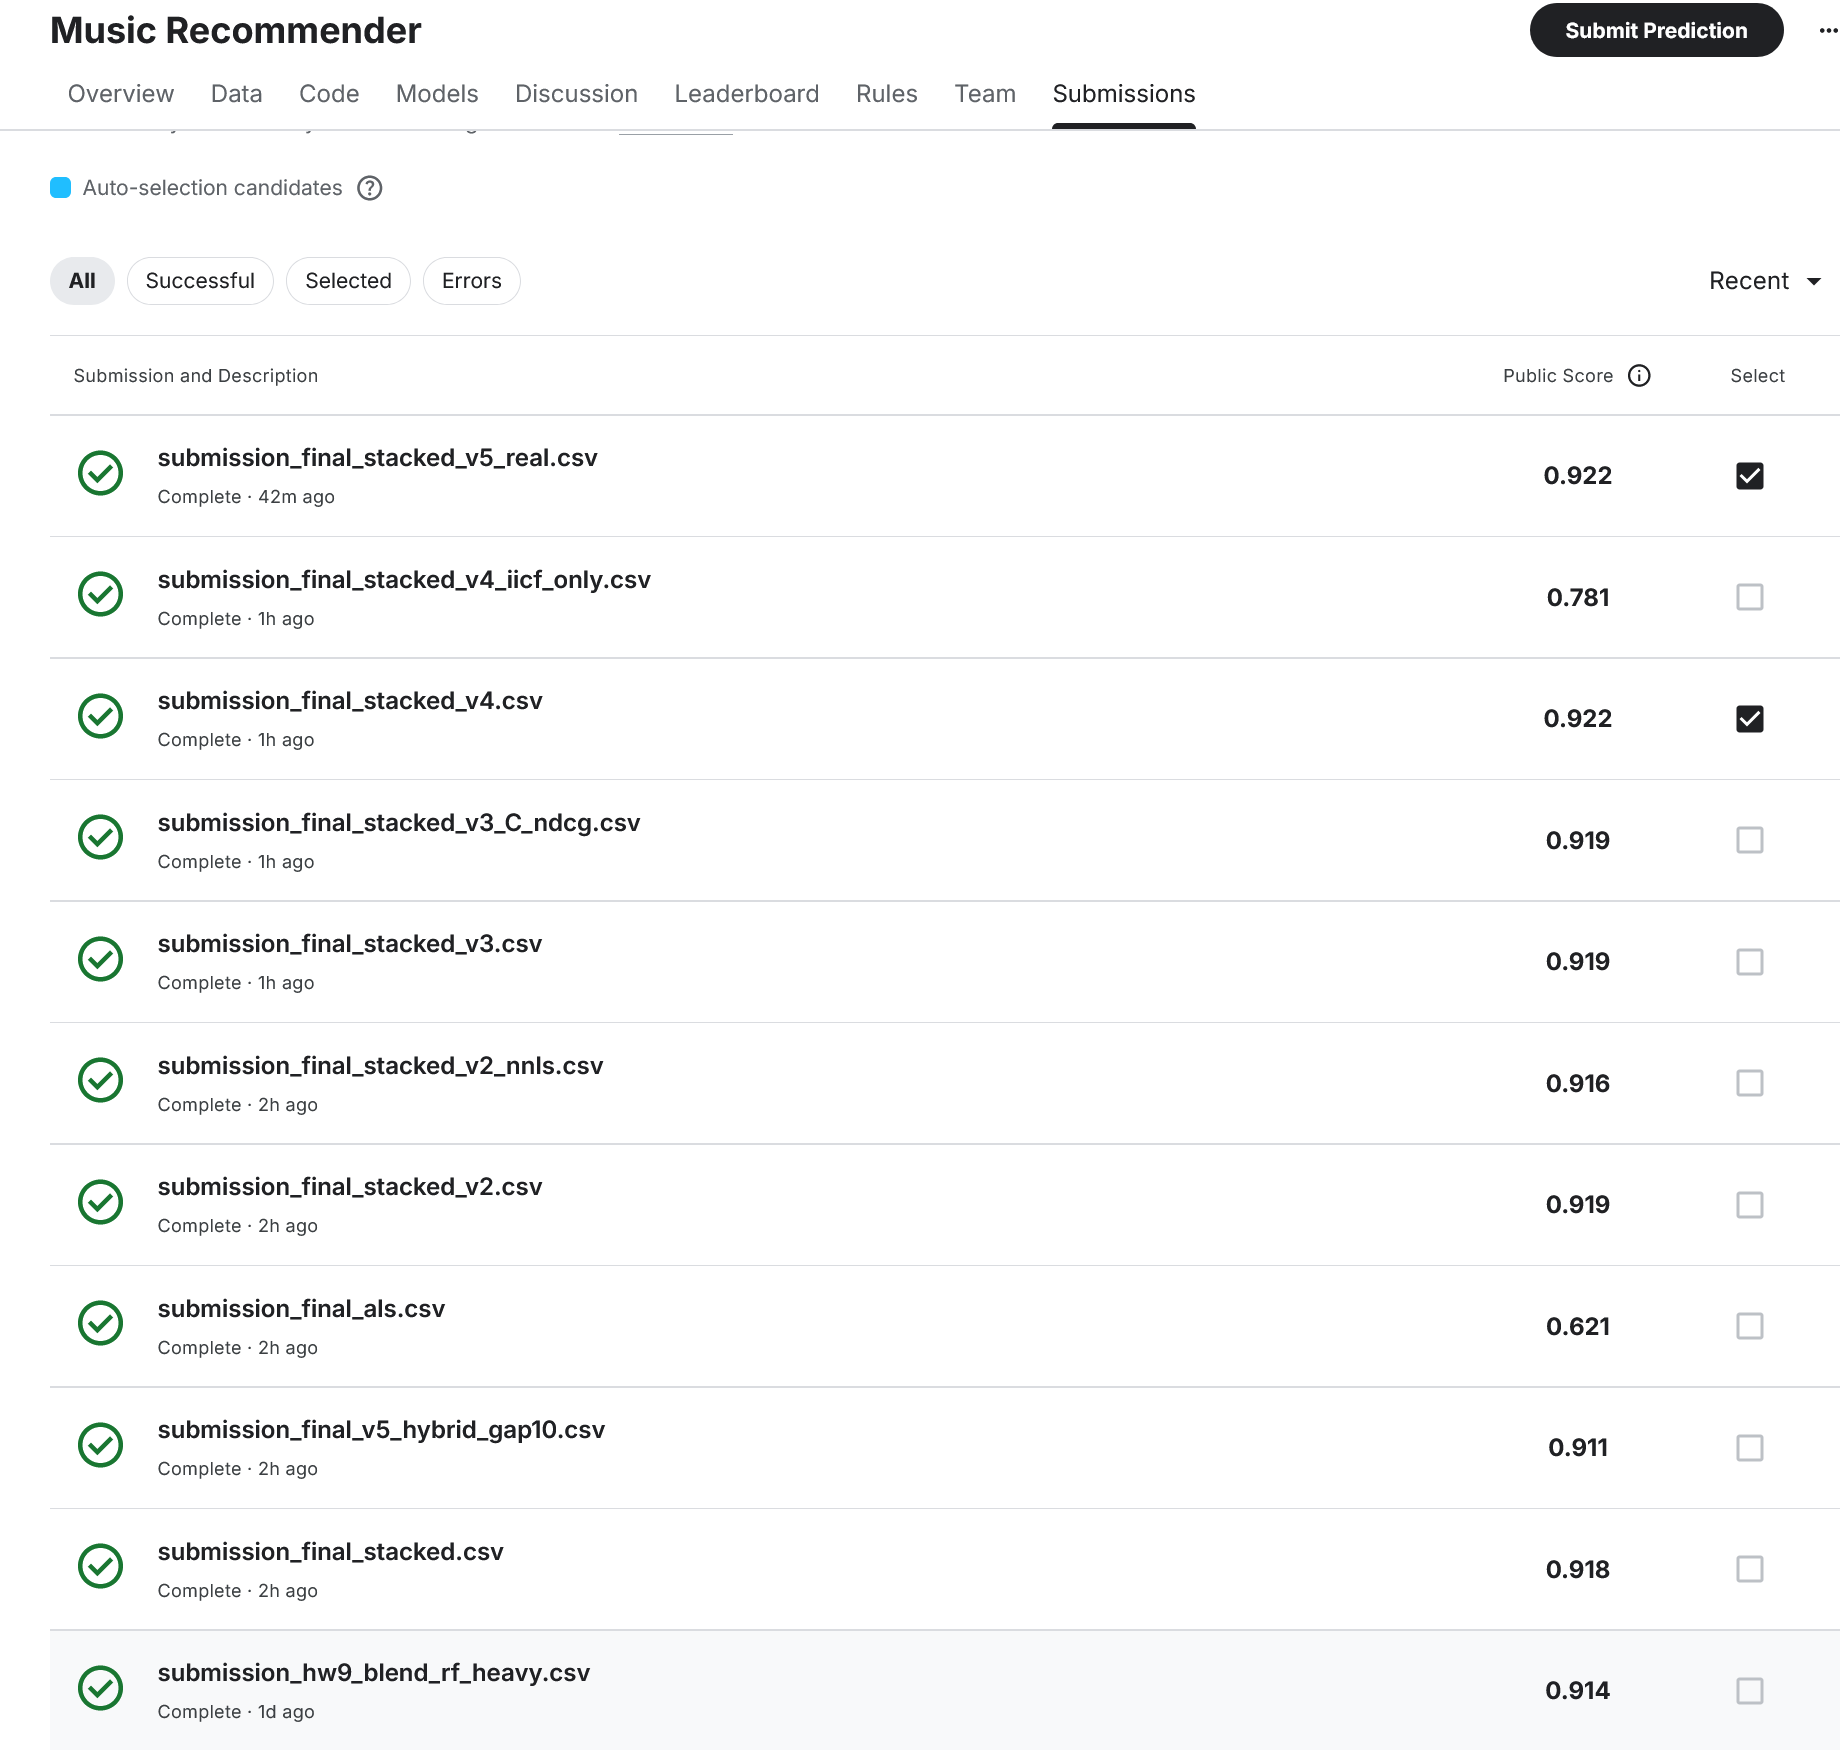
\includegraphics[width=0.95\textwidth]{kaggle_screenshot.png}
		\caption{Kaggle public-leaderboard screenshot showing the final-project submissions. Best score: $\mathbf{0.922}$ (\texttt{submission\_final\_stacked\_v4.csv} and \texttt{submission\_final\_stacked\_v5\_real.csv}, tied).}\label{fig:kaggle}
	\end{figure}

	\newpage
	%======================================================================
	\section{Conclusion}
	%======================================================================

	\begin{enumerate}
		\item A logistic-regression meta-learner stacked over outputs from every prior assignment in the semester reached Kaggle public score $0.922$, an improvement of $+0.011$ over the midterm production submission ($0.911$) and $+0.008$ over the strongest individual base model from HW9 ($0.914$).
		\item The meta-learner directly implements the Week~12 ensemble preview $\hat{y}_{\text{blend}} = \sum_k w_k \hat{y}^{(k)}$ over $39$ archived prior submissions plus continuous-score outputs from rerun base models. Three engineering additions go beyond the lecture: weights are learned by L2-regularized logistic regression on a held-out labeled set, probability calibration (isotonic regression) is applied to non-binary inputs, and tuning uses GroupKFold-by-user CV to prevent per-user pattern memorization.
		\item The Kaggle score progression $0.918 \rightarrow 0.919 \rightarrow 0.919 \rightarrow 0.922 \rightarrow 0.922$ across five meta-learner iterations demonstrates empirically that meta-learner sophistication has diminishing returns once the base-model set is fixed. The single $+0.003$ Kaggle gain in v4 came from adding a base model trained on a fundamentally different feature representation (item-item CF over the raw rating co-occurrence matrix), not from another round of meta-learner tuning.
		\item Three external methods were attempted from the literature: LightGBM LambdaRank, isotonic regression calibration, and NDCG@3 grouped CV. Of those, only isotonic calibration earned a sustained place in the production stack (and its contribution was within fold-noise). The most informative of the three was LightGBM, which early-stopped at iteration~1 because the $32$-feature representation it shared with the BPR neural net had been fully saturated---confirming experimentally that algorithmic novelty is not a substitute for representational diversity.
		\item The final's strongest features come from prior coursework. The largest weight in every meta-learner version is \texttt{hw9\_consensus}, the average of the five $0.913$--$0.914$ HW9 blend submissions. Project~1's heuristic, the midterm BPR neural net, and the eleven midterm $v5\!+\!v2$ confidence-gated hybrids all contribute non-trivially. The semester-long practice of keeping every Kaggle submission---not discarding low-scoring ones---is what made the meta-learner viable.
	\end{enumerate}

	\newpage
	%======================================================================
	% References (auto-generated from references.bib via natbib)
	%======================================================================

	\nocite{chapelle2011yahoo,barlow1972isotonic,deshpande2004topn,wang2013ndcg}
	\bibliographystyle{plainnat}
	\bibliography{references}

	\newpage
	%======================================================================
	\section{Appendix: Python Code}\label{sec:code}
	%======================================================================

	\lstinputlisting[caption={\texttt{EE627\_Final\_Eschete.py} --- full pipeline: MF, BPR neural ranker, ALS, item-item CF, and the v1--v5 stackers.},label={lst:code},basicstyle=\ttfamily\tiny]{EE627_Final_Eschete.py}

\end{document}
